\documentclass{article}

\begin{filecontents}{lie.bib}
	@book{Lee,
		author = {Lee, John M.},
		title = {Introduction to Smooth Manifolds},
		year = 2013,
		edition = "Second Edition"
	}
\end{filecontents}
\usepackage[style=authortitle,backend=bibtex]{biblatex}
\addbibresource{lie.bib}

%Paquetes
\usepackage[left=4cm, right=4cm]{geometry}
\usepackage{titlesec}
\usepackage{fancyhdr}
\usepackage{afterpage}
\usepackage{palatino}%Fuente
 \usepackage{eulervm}%Fuente
\usepackage{graphicx}%Imágenes
\usepackage{float}%Imágenes
\usepackage{subcaption}%Imágenes
\usepackage{enumitem}%Listas
\usepackage{parskip}%Espacio entre párrafos
\usepackage{multicol}
\usepackage{amsthm,thmtools,xcolor}
\usepackage{amssymb}%Mate
\usepackage{amsmath}%Mate
\usepackage{tikz}%Mate (diagramas)
\usepackage{dutchcal}
\usepackage{tikz-cd}
\usepackage{xcolor}
\definecolor{blue-violet}{rgb}{0.54, 0.17, 0.89}
\usetikzlibrary{%
	matrix,%
	calc,%
	arrows,%
	shapes,
	decorations.markings,backgrounds,calc,intersections
}
\usepackage[bookmarks,bookmarksopen,bookmarksdepth=3]{hyperref}%Links a lugares en el texto
\hypersetup{%colores
	colorlinks=true,
	urlcolor=blue,
	linkcolor=magenta,
	citecolor=blue,
	filecolor=blue,
	urlbordercolor=white,
	linkbordercolor=white,
	citebordercolor=white,
	filebordercolor=white
}
\usepackage{cleveref}
\Crefname{exercise}{Exercise}{Exercises}

\makeatletter%Hide ToC header
\renewcommand\tableofcontents{%
	\@starttoc{toc}%
}
\makeatother
\makeatletter %Hide section number
\def\@seccntformat#1{%
	\expandafter\ifx\csname c@#1\endcsname\c@section\else
	\csname the#1\endcsname\quad
	\fi}
\makeatother

\newcommand{\fakesection}[1]{%
	\par\refstepcounter{section}% Increase section counter
	\sectionmark{#1}% Add section mark (header)
	\addcontentsline{toc}{section}{\protect\numberline{\thesection}#1}% Add section to ToC
	% Add more content here, if needed.
}
\usepackage{sectsty}
%\sectionfont{\fontsize{12}{20}\selectfont}

\definecolor{blue-violet}{rgb}{0.54, 0.17, 0.89}
\definecolor{azure}{rgb}{0.0, 0.5, 1.0}
\definecolor{green(ncs)}{rgb}{0.0, 0.62, 0.42}
\definecolor{forestgreen}{rgb}{0.13, 0.55, 0.13}
\definecolor{limegreen}{rgb}{0.2, 0.8, 0.2}
\definecolor{palatinateblue}{rgb}{0.15, 0.23, 0.89}
\definecolor{trueblue}{rgb}{0.0, 0.45, 0.81}
\definecolor{goldenyellow}{rgb}{1.0, 0.87, 0.0}
\definecolor{fashionfuchsia}{rgb}{0.96, 0.0, 0.63}
\definecolor{brightcerulean}{rgb}{0.11, 0.67, 0.84}
\definecolor{jonquil}{rgb}{0.98, 0.85, 0.37}
\definecolor{lavendermagenta}{rgb}{0.93, 0.51, 0.93}
\definecolor{peru}{rgb}{0.8, 0.52, 0.25}
\definecolor{persimmon}{rgb}{0.93, 0.35, 0.0}
\definecolor{persianred}{rgb}{0.8, 0.2, 0.2}
\definecolor{persianblue}{rgb}{0.11, 0.22, 0.73}
\definecolor{persiangreen}{rgb}{0.0, 0.65, 0.58}
\definecolor{persianyellow}{rgb}{0.9, 0.89, 0.0}

%\theoremstyle{definition}

\declaretheoremstyle[headfont=\color{trueblue}\normalfont\bfseries,]{colored1}
\declaretheoremstyle[headfont=\color{forestgreen}\normalfont\bfseries,]{colored2}
\declaretheoremstyle[headfont=\color{peru}\normalfont\bfseries,]{colored3}
\declaretheoremstyle[headfont=\color{persiangreen}\normalfont\bfseries,]{colored4}
\declaretheoremstyle[headfont=\color{brightcerulean}\normalfont\bfseries,]{colored5}
\declaretheoremstyle[headfont=\color{lavendermagenta}\normalfont\bfseries,]{colored6}
\declaretheoremstyle[headfont=\color{blue-violet}\normalfont\bfseries,]{colored7}
\declaretheoremstyle[headfont=\color{green(ncs)}\normalfont\bfseries,]{colored8}
\declaretheoremstyle[headfont=\color{peru}\normalfont\bfseries,]{colored9}
\declaretheoremstyle[headfont=\color{persiangreen}\normalfont\bfseries,]{colored10}

\declaretheorem[style=colored1,numberwithin=section,name=Theorem]{thm}
\declaretheorem[style=colored2,numberwithin=section,numberlike=thm,name=Proposition]{prop}
\declaretheorem[style=colored3,numberwithin=section,numberlike=thm,name=Lemma]{lemma}
\declaretheorem[style=colored4,numberwithin=section,numberlike=thm,name=Corollary]{coro}
\declaretheorem[style=colored5,numbered=no,name=Example]{example}
\declaretheorem[style=colored5,numbered=no,name=Examples]{exemplos}
\declaretheorem[style=colored6,numberwithin=section,name=Exercise]{exercise}
\declaretheorem[style=colored7,numberwithin=section,name=Remark]{remark}
\declaretheorem[style=colored9,numbered=no,name=Claim]{claim}
\declaretheorem[style=colored8,numbered=no,name=Definition]{defn}
\declaretheorem[style=colored10,numbered=no,name=Question]{question}

\numberwithin{equation}{section}

\newcommand{\R}{\mathbb{R}}
\newcommand{\Z}{\mathbb{Z}}
\newcommand{\N}{\mathbb{N}}
\newcommand{\C}{\mathbb{C}}
\newcommand{\Q}{\mathbb{Q}}
\newcommand{\D}{\mathbb{D}}
\newcommand{\T}{\mathbb{T}}
\renewcommand{\P}{\mathbb{P}}
\newcommand{\Ac}{\mathcal{A}}
\newcommand{\Bc}{\mathcal{B}}
\newcommand{\Cc}{\mathcal{C}}
\newcommand{\Dc}{\mathcal{D}}
\newcommand{\Ec}{\mathcal{E}}
\newcommand{\Fc}{\mathcal{F}}
\newcommand{\Gc}{\mathcal{G}}
\newcommand{\Lc}{\mathcal{L}}
\newcommand{\Oc}{\mathcal{O}}
\newcommand{\Qc}{\mathcal{Q}}
\newcommand{\Sc}{\mathcal{S}}
\newcommand{\Wc}{\mathcal{W}}
\newcommand{\mf}{\mathfrak{m}}
\newcommand{\gf}{\mathfrak{g}}
\newcommand{\X}{\mathfrak{X}}
\newcommand{\hf}{\mathfrak{h}}
\newcommand{\glf}{\mathfrak{gl}}
\newcommand{\of}{\mathfrak{o}}

\renewcommand{\Im}{\operatorname{Im}}
\renewcommand{\O}{\operatorname{O}}
\renewcommand{\S}{\mathbb{S}}
\renewcommand{\T}{\mathbb{T}}
\DeclareMathOperator{\Lie}{\operatorname{Lie}}

\DeclareMathOperator{\img}{img}
\DeclareMathOperator{\Arg}{Arg}
\DeclareMathOperator{\End}{End}
\DeclareMathOperator{\id}{id}
\DeclareMathOperator{\Alt}{Alt}
\DeclareMathOperator{\sgn}{sgn}
\DeclareMathOperator{\supp}{supp}
\DeclareMathOperator{\Int}{Int}
\DeclareMathOperator{\Ob}{Ob}
\DeclareMathOperator{\Mor}{Mor}
\DeclareMathOperator{\Top}{Top}
\DeclareMathOperator{\CGWH}{CGWH}
\DeclareMathOperator{\Hom}{Hom}
\DeclareMathOperator{\Map}{Map}
\DeclareMathOperator{\Tot}{Tot}
\DeclareMathOperator{\Vect}{Vect}
\DeclareMathOperator{\VectBund}{VectBund}
\DeclareMathOperator{\Open}{Open}
\DeclareMathOperator{\Ring}{Ring}
\DeclareMathOperator{\Set}{Set}
\DeclareMathOperator{\GL}{GL}
\DeclareMathOperator{\SL}{SL}
\DeclareMathOperator{\SO}{SO}
\DeclareMathOperator{\U}{U}
\DeclareMathOperator{\SU}{SU}
\DeclareMathOperator{\Sp}{Sp}
\DeclareMathOperator{\M}{M}

\pagestyle{empty}
\fancyhf{}
\cfoot{}
\rhead{Daniel González Casanova Azuela}
\lhead{Complex manifolds in dimension 1}
\begin{document}
{\LARGE\bfseries lie groups and lie algebras}
\thispagestyle{fancy}
\vspace{.5cm}

This is just J. Lee, \textit{Introduction to smooth manifolds}, Second Edition.

\tableofcontents
\section{classical lie groups}
\begin{defn}
	A \textbf{\textit{Lie group}} is a smooth manifold $G$ without boundary that is also a group in the algebraic sense, with the property that the multiplication map and the inversion map are both smooth.
\end{defn}
\begin{example}\leavevmode
	\begin{enumerate}
		\item The \textbf{\textit{general linear group}} $\GL(n,\R)$ is the set of invertible $n\times n$ matrices with real entries.
		\item $\GL^+(n,\R)$, the subset of $\GL(n,\R)$ consisting of matrices with positive determinant.
		\item If $G$ is any Lie group and $H\subset G$ is an open subgroup, $H$ is a Lie group (because restrictions of the operations are smooth).
		\item The \textbf{\textit{complex generar linear group}} $\GL(n,\C)$.
		\item If $V$ is any real or complex vector space, $\GL(V)$ denotes que set of invertible linear maps from $V$ to itself. If $V$ is finite dimensional, there is an isomorphism with either of $GL(n,\R)$ or $\GL(n,\C)$.
		\item $\R^n$ and $\C^n$.
		\item The set $\R^*$ of nonzero real numbers. In fact, it is $\GL(1,\R)$. Also $\C^*$.
		\item The circle $\S^1$.
		\item Direct product of Lie groups.
		\item The $n$-torus $\T^n$.
		\item Any discrete group.
		\item The set $\SL(n,\R)$ of $n\times n$ real matrices with determinant equal to 1 is called the \textbf{\textit{special linear group of degree $n$}}. It is the kernel of the group homomorphism $\det:\GL(n,\R)\to\R^*$. Because the determinan function is surjective, it is a smooth submersion by the global rank theorem so $\SL(n,\R)$ has dimension $n^2-1$.
		\item Let $n$ be a positive integer and define the map $\beta:\GL(n,\C)\to\GL(2n,\R)$ by replacing each complex matrix entry by a $2\times 2$ block matrix. Thus $\GL(n,\C)$ is isomorphic to a Lie subgroup of $\GL(2n,\R)$.
		\item The subgroup $\SL(n,\C)\subseteq\GL(n,\C)$ consisting of complex matrices of determinant 1 is called the \textbf{\textit{complex special linear group of degree $n$}}. By similar arguments the real case, it is of codimension $\dim\C^*=2$ and therefore of dimension $2n^2-2$.
		\item A real $n\times n$ matrix $A$ is said to be \textbf{\textit{orthogonal}} if as a linear map it preserves the Euclidean dot product. The set $\O(n)$ of orthogonal $n\times n$ matrices is a subgroup of $\GL(n,\R)$ called the \textbf{\textit{orthogonal group of degree $n$}}. A matrix $A$ is orthogonal if and only if it takes the standard basis of $\R^n$ to an orthonormal basis, which is equivalent to the columns of $A$ being orthonormal. Since the $(i,j)$-entry of the matrix $A^TA$ is the dot product of the $i$th and $j$th columns of $A$, this condition is also equivalent to the requirement that $A^TA=I_n$. Also, $\O(n)$ is the level set $\Phi^{-1}(I_n)$ of the map $\Phi:\GL(n,\R)\to\operatorname{M}(n,\R)$ given by $A\mapsto A^TA$, so it is a closed set and an embedded Lie subgroup. It is also bounded because every $A\in\O(n)$ has colomuns of norm 1, and therefore satisfies that $|A|=\sqrt{n}$. It has dimension $n(n-1)/2$.
		\item The \textbf{\textit{special orthogonal group of degree $n$}} is defined as $\SO(n)=\O(n)\cap\SL(n,\R)\subseteq\GL(n,\R)$. Notice that every matrix $A\in\O(n)$ satisfies
		\[1=\det I_n=\det(A^TA)=\det A\det A^T=(\det A)^2,\]
		it follows that $\det A=\pm1$. Therefore $\SO(n)$ is the open subgroup of $\O(n)$ consisting of matrices with positive determinant, and is therefore also an embedded Lie subgroup of dimension $n(n-1)/2$ in $\GL(n,\R)$. It is a compact group because it is a closed subset of $\O(n)$.
		\item For any complex matrix $A$, the \textbf{\textit{adjoint of $A$}} is the matrix $A^*$ formed by conjugating the entries of $A$ and taking the transpose: $A^*=\overline{A}^T$. For any positive integer $n$, the \textbf{\textit{unitary group of degree $n$}} is the subgroup $\U(n)\subseteq\GL(n,\C)$ consisting of complex $n\times n$ matrices whose columns form an orthogonal basis for $\C^n$ with respect to the Hermitian dot product $z\cdot w=\sum_iz^i\overline{w^i}$. It is straightforward to check that $\U(n)$ consists of those matrices $A$ such that $A^*A=I_n$. It is a properly embedded Lie subgroup of $\GL(n,\C)$ of dimension $n^2$.
		\item The group $\SU(n)=\U(n)\cap\SL(n,\C)$ is called the \textbf{\textit{complex special unitary group of degree $n$}}. It is a properly embedded Lie subgroup of $\U(n)$ of dimension $n^2-1$. It is also embedded in $\GL(n,\C)$ because composition of embedddings is an embedding.
		\item The \textbf{\textit{real symplectic group}} is the subgroup $\Sp(2n,\R)\subseteq\GL(2n,\R)$ consisting of all $2n\times2n$ matrices that leave the standard symplectic tensor $\omega=\sum_{i=1}^ndx^i\wedge dy^i$ invariant, that is, the set of invertible linear maps $Z:\R^{2n}\to\R^{2n}$ such that $\omega(Zx,Zy)=\omega(x,y)$ for all $x,y\in\R^{2n}$.
	\end{enumerate}
\end{example}
\begin{defn}[Extra]
	If $G$ is any Lie group, a \textbf{\textit{(finite-dimensional) representation of $G$}} is a Lie group homomorphism grom $G$ to $\GL(V)$ for some $V$. If a representation is injective, it is said to be \textbf{\textit{faithful}}.
\end{defn}
\section{the lie algebra of a lie group}
Suppose $G$ is a Lie group. Recall that $G$ acts smoothly and transitevely on itself by left translation $L_g(h)=gh$. A vector field $X$ on $G$ is said to be \textbf{\textit{left-invariant}} if it is invariant under all left translations:
\[d(L_g)_{g'}(G_{g'})=X_{gg'}\qquad\text{ for all }g,g'\in G.\]
Since $L_g$ is a diffeomorphism, the pushforward of a vector field is well defined and we may write our condition as $(L_g)_*X=X$ for every $g\in G$.

Because $(L_g)_*(aX+bY)=a(L_g)_*+b(L_g)_*$, the set of left-invariant vector fields on $G$ is a linear subspace of $\X(G)$. But there's more
\begin{prop}
	Let $G$ be a Lie group and suppose that $X$ and $Y$ are left-invariant vector fields on $G$. Then $[X,Y]$ is also left-invariant.
\end{prop}
\begin{defn}
	A \textbf{\textit{Lie algebra}} (over $\R$) is a real vector space $\gf$ endowed with a map called the \textbf{\textit{bracket}} from $\gf\times\gf$ to $\gf$ usually denoted by $(X,Y)\mapsto[X,Y]$ that satisfies the following properties for all $X,Y,Z\in\gf$:
	\begin{enumerate}
		\item {\scshape Bilinearity:} For $a,b\in\R$,
		\[[aX+bY,Z]=a[X,Z]+b[Y,Z],\]
		\[[Z,aX+bY]=a[Z,X]+b[Z,Y].\]
		\item {\scshape Antisymmetry:}
		\[[X,Y]=-[Y,X].\]
		\item {\scshape Jacobi Identity:}
		\[[X,[Y,Z]]+[Y,[Z,X]]+[Z,[X,Y]]=0.\]
	\end{enumerate}
\end{defn}
Notice that the Jacobi identity is a substitute for associativity, which does not hold in general for brackets in a Lie algebra. We may also define Lie algebras over $\C$.
\begin{defn}\leavevmode
	\begin{itemize}
		\item If $\gf$ is a Lie algebra, a linear subspace $\hf\subseteq\gf$ is called a \textbf{\textit{Lie subalgebra of $\gf$}} if it is closed under brackets.
		\item If $\gf$ and $hf$ are Lie algebras, a linear map $A:\gf\to\hf$ is called a \textbf{\textit{Lie algebra homomorphism}} if it preserves brackets: $A[X,Y]=[AX,AY]$. An invertible Lie algebra homomorphism is called a \textbf{\textit{Lie algebra isomorphism}}.
	\end{itemize}
\end{defn}
\begin{example}\leavevmode
	\begin{enumerate}
		\item The space $\X(M)$ of all smooth vector fields on a smooth manifold $M$ is a Lie algebra under the Lie bracket.
		\item If $G$ is a Lie group, the set of all left-invariant vector fields on $G$ is a Lie subalgebra of $\X(G)$. This is called the \textbf{\textit{Lie algebra of $G$}} and it is denoted by $\Lie(G)$.
		\item The vector space $\M(n,\R)$ of $n\times n$ real matrices is an $n^2$-dimensional Lie algebra under the \textbf{\textit{commutator bracket}}
		\[[A,B]=AB-BA.\]
		When regarding $\M(n,\R)$ as a Lie algebra with this bracket, we denote it by $\glf(n,\R)$.
		\item Similarly, $\glf(n,\C)$ is the $2n^2$-dimensional (real) Lie algebra obtained by endowing $\M(n,\C)$ with the commutator bracket.
		\item If $V$ is a vector space, the vector space of all linear maps from $V$ to itself becomes a Lie algebra which we denote $\glf(V)$ with the commutator bracket:
		\[[A,B]=A\circ B-B\circ A.\]
		Under the usual identification of $n\times n$ matrices with linear maps from $\R^n$ to itself, $\glf(\R^n)$ is the same as $\glf(n,\R)$.
		\item Any vector space $V$ becomes a lie algebra if we define all brackets to be zero. Such a Lie algebra is said to be \textbf{\textit{abelian}}.
	\end{enumerate}
\end{example}
\begin{thm}
	Let $G$ be a Lie group. The evaluation map $\varepsilon:\Lie(G)\to T_eG$ given by $\varepsilon(X)=X_e$ is a vector space isomorphism. Thus $\Lie(G)$ is finite-dimensional with dimension equal to $\dim G$.
\end{thm}
\begin{coro}
	Every left-invariant rough vector field on a Lie group is smooth.
\end{coro}
\begin{coro}
	Every Lie group admits a left-invariant smooth global frame, and therefore every Lie group is parallelizable.
\end{coro}
\begin{example}\leavevmode
	\begin{enumerate}
		\item $\Lie(\R^n)\cong\R^n$.
		\item $\Lie(\S^1)\cong\R$.
		\item $\Lie(\T^n)\cong\R^n$.
		\item $\Lie(\GL(n,\R))\cong\glf(n,\R)$. (long proof)
		\item If $V$ is any finite-dimensional real vector space, $\Lie(\GL(V))\cong\glf(V)$.
		\item $\Lie(\GL(n,\C))\cong\glf(n,\C)$.
		\item $\of(n)=\{\text{skew-symmetric }n\times n\text{ matrices}\}\subseteq\glf(n,\R)$ is $\Lie(\O(n))$.
		\item $\Lie(\GL(n,\C))\cong\glf(n,\C)$. (long proof)
	\end{enumerate}
\end{example}
\begin{thm}[Ado's Theorem]
	Every finite-dimensional real Lie algebra admits a faithful finite-dimensional representation.
\end{thm}
\begin{coro}
	Every finite-dimensional real Lie algebra is isomorphic to a Lie subalgebra of some matrix algebra $\glf(n,\R)$ with the commutator bracket.
\end{coro}

\section{the exponential map}
\begin{defn}
	Suppose $G$ is a Lie group. A \textbf{\textit{one-parameter subgroup of $G$}} is defined to be a Lie group homomorphism $\gamma:\R\to G$ with $R$ considered as a lie group under addition. Notice that by this definition, a one-parameter subgroup is not a Lie subgroup of $G$ but rather a homomorphism into $G$.
\end{defn}
\begin{thm}
	The one-parameter subgroups of $G$ are precisely the maximal integral curves of left-invariante vector fields starting at the identity.
\end{thm}
\begin{defn}
	Given $X\in\Lie(G)$, the one-parameter subgroup determined by $X$ in this way is called the \textbf{\textit{one-parameter subgroup generated by $X$}}.
\end{defn}
Because left-invariant vector fields are uniquely determined by their values at the identity, it follows that each one-parameter subgroup is unequely determined by its initial velocity in $T_eG$, and thus there are one-to-one correspondences
\[\{\text{one-parameter subgroups of }G\}\leftrightarrow\Lie(G)\leftrightarrow T_eG.\]
\begin{prop}
	For any $A\in\glf(n,\R)$, let
	\[e^A=\sum_{k=0}^\infty\frac{1}{k!}A^k=I_n+A+\frac{1}{2}A^2+\ldots.\]
	This series converges to an invertible matrix $e^A\in\GL(n,\R)$ and the one-parameter subgroup of $\GL(n,\R)$ generated by $A\in\glf(n,\R)$ is $\gamma(t)=e^{tA}$.
\end{prop}
\begin{prop}
	Suppose $G$ is a Lie group and $H\subseteq G$ is a Lie subgroup. The one-parameter subgroups of $H$ are precisely those one-parameter subgroups of $G$ whose initial velocities lie in $T_eH$.
\end{prop}
\begin{example}
	If $H$ is a Lie subgroup of $\GL(n,\R)$, the precding proposition shows that the one-parameter subgroups of $H$ are precisely the maps of the form $\gamma(t)=e^{tA}$ for $A\in\hf$, where $h\subseteq\glf(n,\R)$ is the subalgebra cooresponding to $\Lie(H)$. For example, taking $H=\O(n)$ this shows that the one-parameter subgroups of $\O(n)$ are the maps of the form $\gamma(t)=e^{tA)}$ for an arbitrary skew-symmetric $A$. In particular, this shows that the exponential of any skew-symmetric matrix is orthogonal.
\end{example}
\begin{defn}
	Given a Lie group $G$ with Lie algebra $\gf$, we define the map $\exp:\gf\to G$ called the \textbf{\textit{exponential map of $G$}} as follows: for any $X\in\gf$, we set
	\[\exp X=\gamma(1),\]
	where $\gamma$ is the one-parameter subgroup generated by $X$, or equivalently the integral curve of $X$ starting at the identity.
\end{defn}
\begin{figure}
	\centering
	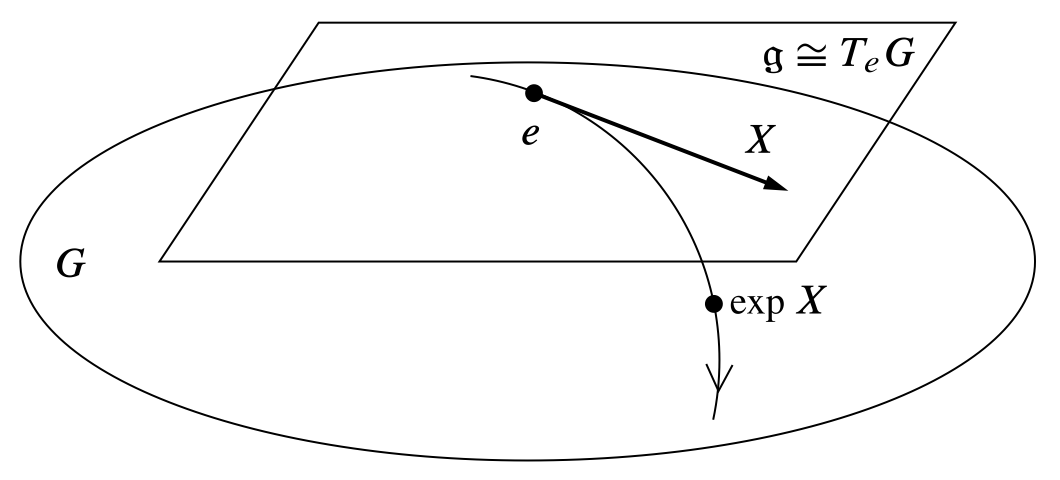
\includegraphics[width=0.7\linewidth]{exp}
	\label{fig:exp}
\end{figure}

\begin{prop}
	Let $G$ be a Lie group. For any $X\in\Lie(G)$, $\gamma(s)=\exp sX$ is the one-parameter subgroup of $G$ generated by $X$.
\end{prop}
\begin{example}\leavevmode
	\begin{enumerate}
		\item $\exp A=e^A$.
		\item If $V$ is any finite-dimensional real vector space, a choice of basis for $V$ yields isomorphisms $\GL(V)\cong\GL(n,\R)$ and $\glf(V)\cong\glf(n,\R)$. The analysis of the $\GL(n,\R)$ case then shows that the exponential map of $\GL(V)$ can be written in the form
		\[\exp A=\sum_{k=0}^\infty\frac{1}{k!}A^k\]
		when we consider $A\in\glf(V)$ as a linear map from $V$ to itself and $A^k=A\circ\ldots\circ A$.
	\end{enumerate}
\end{example}
\begin{prop}
	Let $G$ be a Lie group and $\gf$ be its Lie algebra.
	\begin{enumerate}
		\item The exponential map is a smooth map from $\gf$ to $G$.
		\item For any $X\in\gf$ and $s,t\in\R$, $\exp(s+t)X=\exp sX\exp tX$.
		\item For any $X\in\gf$, $(\exp X)^{-1}=\exp(-X)$.
		\item For any $X\in\gf$ and $n\in\Z$, $(\exp X)^n=\exp(nX)$.
		\item The differential $(d\exp)_0:T_0\gf\to T_eG$ is the identity map, under the canonical identifications of both $T_0\gf$ and $T_eG$ with $\gf$ itself.
		\item The exponential map restricts to a diffeomorphism from some neighborhood of 0 in $\gf$ to a neighborhood of $e$ in $G$.
	\end{enumerate}
\end{prop}
Notice that $\exp(X+Y)=\exp X\exp Y$ for arbitrary $X,Y$ in the Lie algebra. In fact, for connected groups, this is only true when the group is abelian.

\begin{thm}[The Lie correspondence]
	There is a one-to-one correspondence between isomorphism classes of finite-dimensional Lie algebras and isomorphism classes of simply connected Lie groups given by associating each simply connected Lie group with its Lie algebra.
\end{thm}
\end{document}